\documentclass[12pt,aspectratio=169]{beamer}

\usetheme{moloch}
\molochset{progressbar=none, sectionpage=none}

\usepackage[spanish,es-nodecimaldot]{babel}
\usepackage{fontspec}
\usepackage{unicode-math}
\usepackage{graphicx}
\usepackage{booktabs}
\usepackage{array}
\usepackage{amsmath}
\usepackage{ragged2e}
\usepackage{pgfpages}
\usepackage{xurl}

\usefonttheme{professionalfonts}
\setsansfont{Libertinus Sans}[Scale=0.96]
\setmathfont{Libertinus Math}[Scale=MatchLowercase]
\setbeameroption{hide notes}
\graphicspath{{figuras/}}

\definecolor{ink}{HTML}{24313F}
\definecolor{academicgreen}{HTML}{3F6F66}
\definecolor{academicgreenDark}{HTML}{2E4E49}
\definecolor{mutedblue}{HTML}{3F596A}
\definecolor{mutedteal}{HTML}{3F6F66}
\definecolor{mutedbrown}{HTML}{8A7464}
\definecolor{mutedrose}{HTML}{8B6670}
\definecolor{softgray}{HTML}{F3F5F3}
\definecolor{midgray}{HTML}{6F747B}
\definecolor{rulegray}{HTML}{C9D0CC}
\definecolor{footerbg}{HTML}{EDF1EF}

\setbeamercolor{background canvas}{bg=white}
\setbeamercolor{normal text}{fg=ink,bg=white}
\setbeamercolor{frametitle}{fg=ink,bg=white}
\setbeamercolor{title}{fg=ink}
\setbeamercolor{title band}{fg=white,bg=academicgreen}
\setbeamerfont{frametitle}{size=\large,series=\bfseries}
\setbeamerfont{title}{size=\Huge,series=\bfseries}
\setbeamerfont{subtitle}{size=\Large}
\setbeamersize{text margin left=9mm,text margin right=9mm}
\setbeamertemplate{navigation symbols}{}
\setbeamertemplate{footline}{%
  \leavevmode
  \hbox{%
    \begin{beamercolorbox}[wd=.34\paperwidth,ht=2.8ex,dp=1.1ex,leftskip=6mm]{footline left}%
      {\fontsize{5.8}{6.9}\selectfont\bfseries Gutiérrez, Chaves, Miranda y Calderón (UCR)}
    \end{beamercolorbox}%
    \begin{beamercolorbox}[wd=.32\paperwidth,ht=2.8ex,dp=1.1ex,center]{footline center}%
      {\fontsize{5.8}{6.9}\selectfont\bfseries Mortalidad por causa en Centroamérica}
    \end{beamercolorbox}%
    \begin{beamercolorbox}[wd=.34\paperwidth,ht=2.8ex,dp=1.1ex]{footline right}%
      \hbox to .34\paperwidth{\hfill{\fontsize{5.8}{6.9}\selectfont\bfseries 7 jul. 2026 \quad \insertframenumber/10}\hspace{6mm}}
    \end{beamercolorbox}%
  }%
}
\setbeamercolor{footline left}{fg=white,bg=academicgreen}
\setbeamercolor{footline center}{fg=white,bg=academicgreenDark}
\setbeamercolor{footline right}{fg=white,bg=academicgreen}

\newcommand{\sectionrule}{%
  \vspace{1mm}{\color{rulegray}\hrule height 0.5pt}\vspace{2mm}%
}

\newcommand{\smallrule}{%
  {\color{rulegray}\hrule height 0.5pt}\vspace{1.5mm}%
}

\newcommand{\resultline}[2]{%
  {\color{#1}\rule{2.5pt}{0.78cm}}\hspace{2mm}%
  \begin{minipage}[b]{0.88\linewidth}
    {\RaggedRight\normalsize #2}
  \end{minipage}%
}

\newcommand{\charttitle}[1]{%
  \begingroup
  \RaggedRight
  {\fontsize{6.6}{7.4}\selectfont\bfseries #1\par}
  \endgroup
  \vspace{0.8mm}
}

\newcommand{\chartnote}[2]{%
  \par\vspace{0.6mm}
  \begingroup
  \RaggedRight
  {\fontsize{5.1}{5.8}\selectfont Nota: #1\par}
  {\fontsize{5.1}{5.8}\selectfont Fuente: #2\par}
  \endgroup
}

\newcommand{\limitpoint}[2]{%
  \begin{minipage}[t][24mm][t]{0.29\textwidth}
    \centering
    {\fontsize{17}{19}\selectfont\bfseries #1\par}
    \vspace{1.4mm}
    {\color{rulegray}\hrule height 0.5pt}
    \vspace{2mm}
    {\large #2\par}
  \end{minipage}
}

\newcommand{\closingpoint}[3]{%
  \begin{minipage}[t]{0.30\textwidth}
    \RaggedRight
    \hyphenpenalty=10000\exhyphenpenalty=10000\relax
    {\color{#1}\rule{\linewidth}{1.2pt}}
    \vspace{1.2mm}
    {\normalsize\bfseries #2\par}
    \vspace{1mm}
    {\small #3\par}
  \end{minipage}
}

\newcommand{\aparef}[1]{%
  \par\begingroup
  \leftskip=5mm
  \noindent\hspace*{-5mm}#1\par
  \endgroup\vspace{0.16mm}%
}

\newcommand{\qdec}{\ensuremath{q_{x,t}^{(c)}}}
\newcommand{\picausal}{\ensuremath{\pi_{x,t}^{(c)}}}

\title{La causa de muerte cambia la lectura de la mortalidad centroamericana}
\subtitle{Probabilidades de decremento múltiple por causa de muerte en Centroamérica, 2015-2018}
\author{Benjamín Gutiérrez Padua \and Gabriel de Jesús Chaves Esquivel \and Sebastián Miranda Ramírez \and Kevin David Calderón Martínez}
\institute{CA0303 Estadística Actuarial · Universidad de Costa Rica}
\date{Profesor: Maikol Solís Chacón}

\begin{document}

\begin{frame}
  \centering
  \vspace{2mm}
  {\large\color{academicgreenDark} UNIVERSIDAD DE COSTA RICA\par}

  \vspace{5mm}
  \begin{beamercolorbox}[wd=0.92\paperwidth,sep=3.8mm,center]{title band}
    {\fontsize{19}{23}\selectfont\bfseries
    La causa de muerte cambia la lectura de la mortalidad centroamericana\par}
    \vspace{1.5mm}
    {\large Probabilidades de decremento múltiple por causa de muerte en Centroamérica, 2015-2018\par}
  \end{beamercolorbox}

  \vspace{7mm}
  \begin{columns}[T,totalwidth=0.92\paperwidth]
    \begin{column}{0.24\paperwidth}
      \centering
      {\normalsize Sebastián Miranda Ramírez\par}
      {\small C4H274}
    \end{column}
    \begin{column}{0.24\paperwidth}
      \centering
      {\normalsize Gabriel de Jesús Chaves Esquivel\par}
      {\small C4E273}
    \end{column}
    \begin{column}{0.22\paperwidth}
      \centering
      {\normalsize Kevin David Calderón Martínez\par}
      {\small C4D511}
    \end{column}
    \begin{column}{0.22\paperwidth}
      \centering
      {\normalsize Benjamín Gutiérrez Padua\par}
      {\small C4F813}
    \end{column}
  \end{columns}
  \note{Sebastián. Abrimos con la idea central: en mortalidad no basta una cifra total. Dos poblaciones pueden tener niveles parecidos de mortalidad y aun así morir por causas muy distintas, en edades distintas y con diferencias por sexo y país. La charla va a defender que el marco de decrementos múltiples permite leer esa estructura causal en Centroamérica. No vamos a recorrer todo el informe; vamos a quedarnos con los resultados que sostienen mejor esa idea.}
\end{frame}

\begin{frame}{Una tasa agregada aplana diferencias que sí importan}
  \vspace{3mm}
  \begin{columns}[c,totalwidth=0.94\textwidth]
    \begin{column}{0.42\textwidth}
      \centering
      {\large\bfseries Mortalidad total}

      \vspace{6mm}
      {\setlength{\fboxsep}{0pt}\setlength{\fboxrule}{0.8pt}
      \fcolorbox{rulegray}{white}{%
        \textcolor{mutedblue}{\rule{3.6cm}{0.62cm}}%
        \textcolor{softgray}{\rule{0.65cm}{0.62cm}}}}

      \vspace{3mm}
      {\large una sola cifra}
    \end{column}

    \begin{column}{0.10\textwidth}
      \centering
      {\Large\color{mutedbrown}\(\ne\)}
    \end{column}

    \begin{column}{0.42\textwidth}
      \centering
      {\large\bfseries Mortalidad por causa}

      \vspace{5mm}
      \textcolor{mutedteal}{\rule{2.0cm}{0.20cm}}\\[1.5mm]
      \textcolor{mutedbrown}{\rule{1.45cm}{0.20cm}}\\[1.5mm]
      \textcolor{mutedblue}{\rule{1.05cm}{0.20cm}}\\[1.5mm]
      \textcolor{mutedrose}{\rule{0.70cm}{0.20cm}}

      \vspace{3mm}
      {\large edad, país, sexo y año}
    \end{column}
  \end{columns}

  \vspace{8mm}
  \centering
  {\large\bfseries ¿Qué patrones aparecen en \qdec{} por causa ICD-10?}

  \note{Sebastián. El problema es que una tasa agregada parece limpia, pero borra la estructura que queremos estudiar. La pregunta del proyecto no es solo dónde hay más defunciones, sino cómo cambia la probabilidad de decremento por causa cuando movemos edad, país, sexo y año. Esta filmina prepara la necesidad de la celda actuarial: si queremos interpretar causas competidoras, necesitamos conservar esas dimensiones desde el inicio.}
\end{frame}

\begin{frame}{La unidad de análisis conserva cinco dimensiones}
  \centering
  {\fontsize{18}{22}\selectfont\bfseries
  país \(\times\) sexo \(\times\) año \(\times\) edad \(\times\) causa ICD-10}

  \vspace{6mm}
  \begin{tabular}{@{}p{0.25\textwidth}p{0.56\textwidth}@{}}
    \toprule
    \bfseries Observa & \(D_{x,t}^{(c)}\) defunciones y \(E_{x,t}\) exposición\\
    \midrule
    \bfseries Alcance & 6 países, 2015-2018\\[1.3mm]
    \bfseries Causas & Clasificación ICD-10\\[1.3mm]
    \bfseries Insumos & OMS y WPP 2024\\
    \bottomrule
  \end{tabular}

  \note{Gabriel. La unidad de trabajo no es una persona individual, sino una celda agregada. Cada celda combina país, sexo, año, grupo etario y causa ICD-10. Para esa celda tenemos conteos de defunciones y una exposición poblacional común. Con eso podemos pasar de una base descriptiva a una lectura actuarial. También marcamos el alcance: seis países, 2015 a 2018, y Honduras fuera por compatibilidad de información en el periodo.}
\end{frame}

\begin{frame}{El modelo convierte conteos en decrementos anuales}
  \begin{columns}[T,totalwidth=\textwidth]
    \begin{column}{0.30\textwidth}
      \centering
      {\large\bfseries Datos}
      \sectionrule
      {\fontsize{21}{25}\selectfont \(D_{x,t}^{(c)},\,E_{x,t}\)}
    \end{column}
    \begin{column}{0.31\textwidth}
      \centering
      {\large\bfseries Estimación}
      \sectionrule
      {\Large Clásico}

      \vspace{1mm}
      {\Large Bayes}
    \end{column}
    \begin{column}{0.31\textwidth}
      \centering
      {\large\bfseries Salidas}
      \sectionrule
      {\fontsize{21}{25}\selectfont \(\qdec,\,\picausal\)}
    \end{column}
  \end{columns}

  \vspace{7mm}
  \centering
  {\Large
  \[
    q_{x,t}^{(c)} = P(T_{x,t}\leq 1,\ J=c)
  \]
  }

  \note{Gabriel. La metodología se puede contar en tres piezas. Partimos de defunciones y exposición. Eso se convierte en una probabilidad anual de decremento por causa y en una composición causal condicionada al fallecimiento. La fórmula que mostramos es solo la definición del objeto actuarial: la probabilidad de salir del estado vivo durante un año por la causa c. El enfoque clásico estima directamente; el bayesiano usa información colectiva para suavizar celdas sensibles.}
\end{frame}

\begin{frame}{Las causas externas se concentran en hombres jóvenes}
  \begin{columns}[T,totalwidth=\textwidth]
    \begin{column}{0.64\textwidth}
      \charttitle{Gráfico 1. Probabilidad de decremento por causas externas en hombres de 20 a 24 años, según país, 2015 y 2018}
      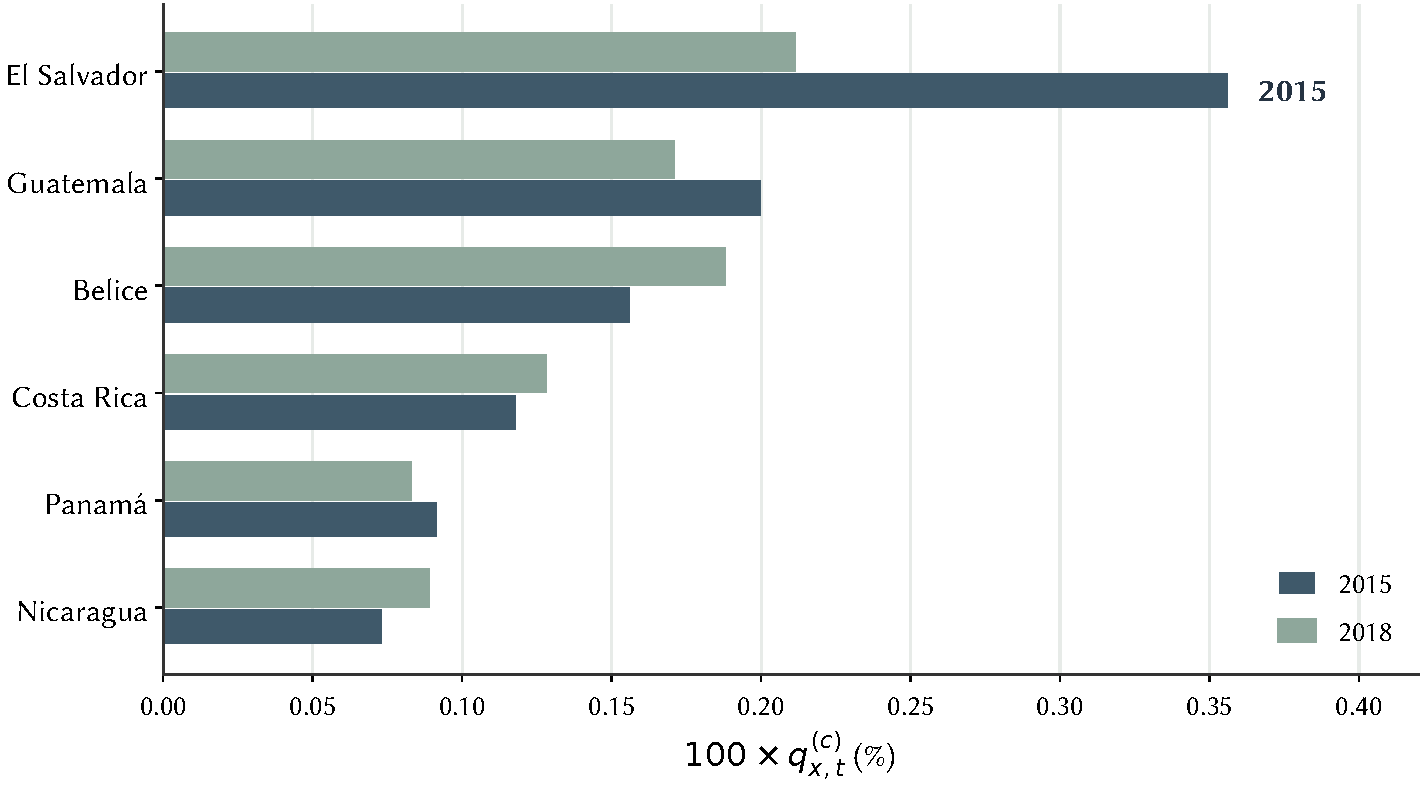
\includegraphics[height=0.42\paperheight,width=\linewidth,keepaspectratio]{externas_hombres_20_24.pdf}
      \chartnote{Valores expresados como \(100\times q_{x,t}^{(c)}\).}{Elaboración propia con datos de la OMS (WHO Mortality Database) y Naciones Unidas (WPP 2024).}
    \end{column}
    \begin{column}{0.30\textwidth}
      \RaggedRight
      \vspace{3mm}
      {\large\bfseries El Salvador}

      \vspace{3mm}
      \resultline{mutedblue}{92.6\,\%\\sobre la mediana}

      \vspace{3mm}
      {\normalsize hombres 20-24}
    \end{column}
  \end{columns}
  \note{Kevin. Este es el primer resultado fuerte. Las causas externas no dominan la mortalidad total de la región, pero sí aparecen con mucha fuerza en edades jóvenes, especialmente en hombres. En el documento final se reporta que El Salvador concentró 92.6\% de las muertes por agresiones dentro del conjunto de países sobre la mediana. La gráfica muestra la señal en hombres de 20 a 24 años: El Salvador sobresale en 2015 y luego baja en 2018. La transición es natural: ahora pasamos del patrón joven a la estructura crónica de edades avanzadas.}
\end{frame}

\begin{frame}{La mortalidad circulatoria gana peso en edades avanzadas}
  \vspace{-4mm}
  \begin{columns}[T,totalwidth=\textwidth]
    \begin{column}{0.68\textwidth}
      \charttitle{Gráfico 2. Probabilidad local de decremento por enfermedades circulatorias en hombres de 65 a 69 años, según país, 2015 y 2018}
      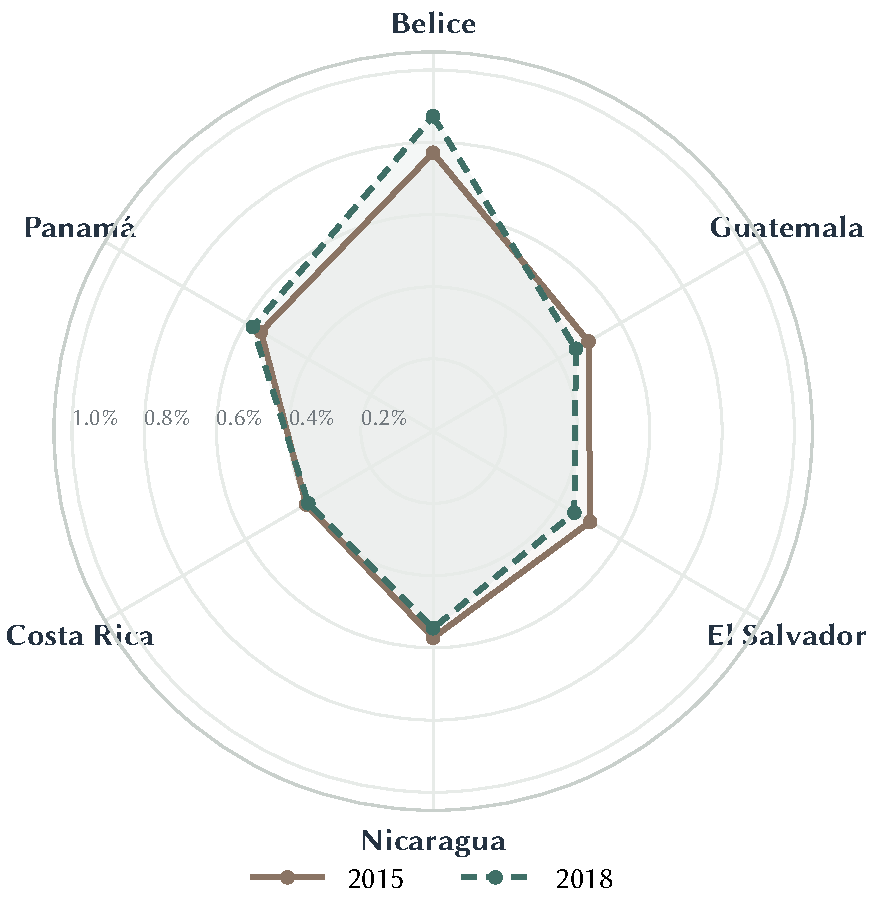
\includegraphics[height=0.55\paperheight,width=\linewidth,keepaspectratio]{radar_circulatorio_hombres_65_69.pdf}
      \chartnote{Valores expresados como \(100\times q_{x,t}^{(c)}\).}{Elaboración propia con datos de la OMS (WHO Mortality Database) y Naciones Unidas (WPP 2024).}
    \end{column}
    \begin{column}{0.26\textwidth}
      \RaggedRight
      \vspace{11mm}
      {\large\bfseries Belice}

      \vspace{3mm}
      \resultline{mutedteal}{nivel local más alto}

      \vspace{3mm}
      {\normalsize hombres 65-69}
    \end{column}
  \end{columns}
  \note{Kevin. El segundo resultado es el contrapunto demográfico: al avanzar la edad, las causas crónicas, especialmente las enfermedades del sistema circulatorio, ganan peso. El informe final destaca el caso de Belice en hombres de 65 a 69 años, donde la probabilidad local por sistema circulatorio sube de 2015 a 2018 y queda como el nivel más alto dentro de esa celda. No lo vamos a presentar como tendencia regional, porque el periodo es corto; lo importante es que la mortalidad por causa se lee en celdas específicas.}
\end{frame}

\begin{frame}{La composición causal cambia claramente con la edad}
  \vspace{-4mm}
  \begin{columns}[T,totalwidth=\textwidth]
    \begin{column}{0.69\textwidth}
      \charttitle{Gráfico 3. Composición causal promedio por edad en Costa Rica}
      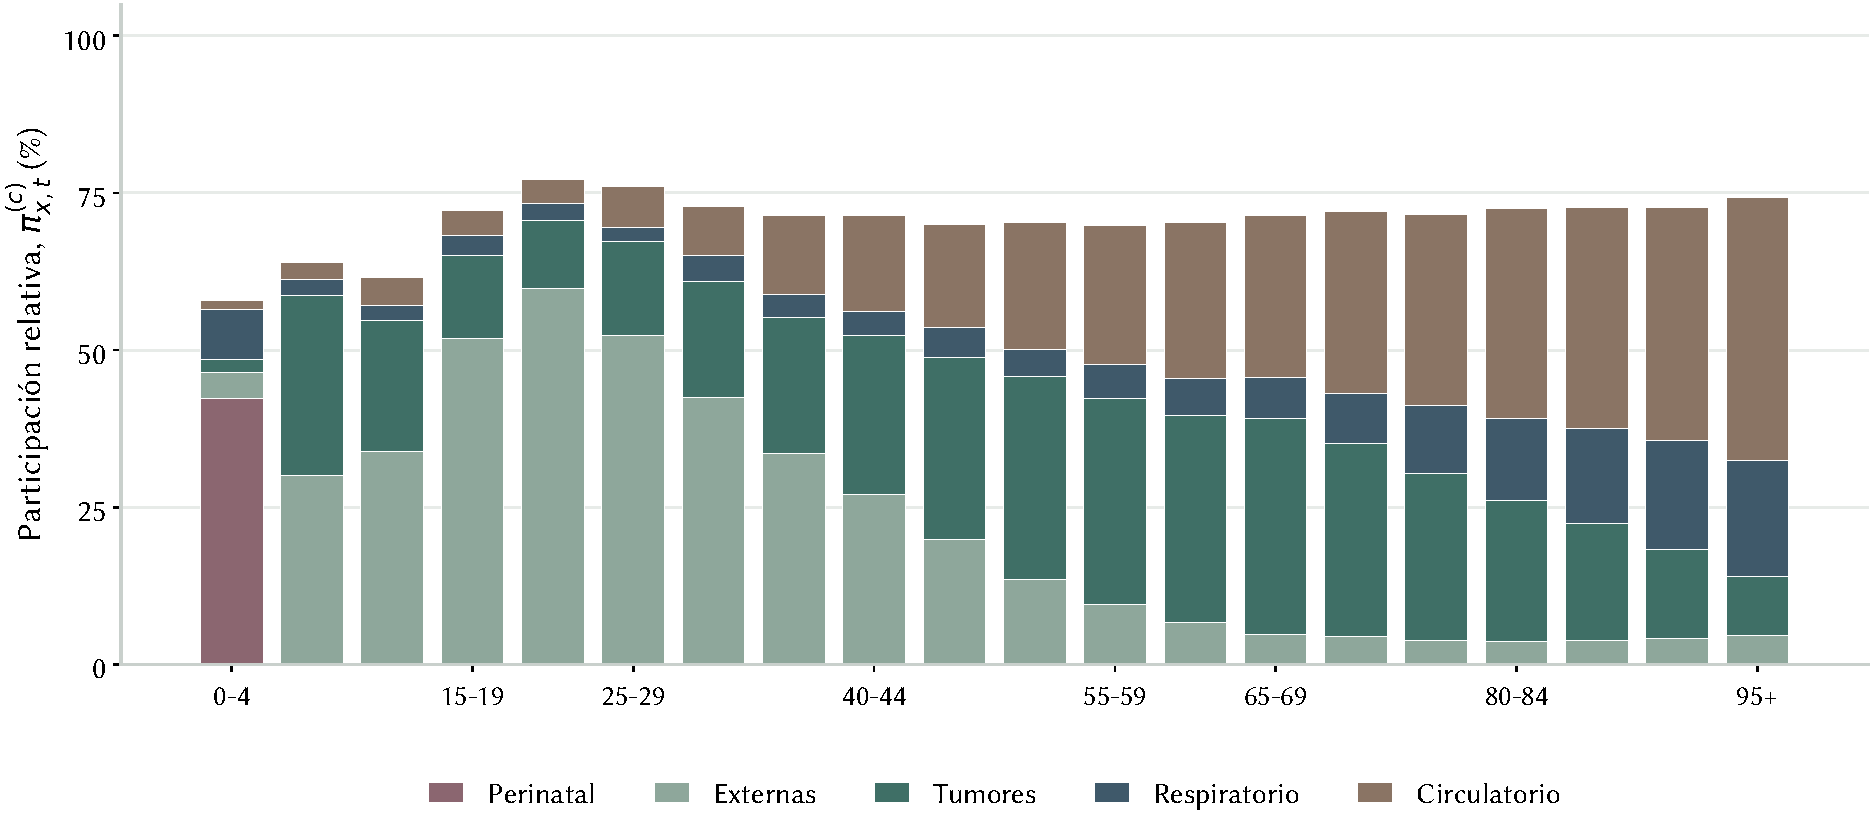
\includegraphics[height=0.46\paperheight,width=\linewidth,keepaspectratio]{composicion_costa_rica_edad.pdf}
      \chartnote{Los porcentajes corresponden a la composición causal \(\pi_{x,t}^{(c)}\), condicionada al fallecimiento.}{Elaboración propia con datos de la OMS (WHO Mortality Database) y Naciones Unidas (WPP 2024).}
    \end{column}
    \begin{column}{0.26\textwidth}
      \RaggedRight
      \vspace{9mm}
      {\large\bfseries Costa Rica}

      \vspace{3mm}
      \resultline{mutedrose}{perinatal al inicio}

      \vspace{2.5mm}
      \resultline{mutedteal}{externas en jóvenes}

      \vspace{2.5mm}
      \resultline{mutedbrown}{circulatorio al final}

      \vspace{4mm}
      {\normalsize lectura de \picausal}
    \end{column}
  \end{columns}
  \note{Kevin. Esta figura viene del análisis del informe, simplificada para presentación. En Costa Rica, la composición causal cambia con la edad: las causas perinatales aparecen al inicio, las causas externas ganan peso en edades jóvenes y la mortalidad circulatoria se vuelve más importante en edades avanzadas. Esta es una lectura de \(\pi_{x,t}^{(c)}\), no de riesgo absoluto: muestra cómo se reparten las defunciones observadas entre causas.}
\end{frame}

\begin{frame}{El suavizamiento bayesiano pesa más en celdas con pocos eventos}
  \begin{columns}[T,totalwidth=\textwidth]
    \begin{column}{0.64\textwidth}
      \charttitle{Gráfico 4. Discrepancia relativa entre el enfoque clásico y el bayesiano, causas seleccionadas}
      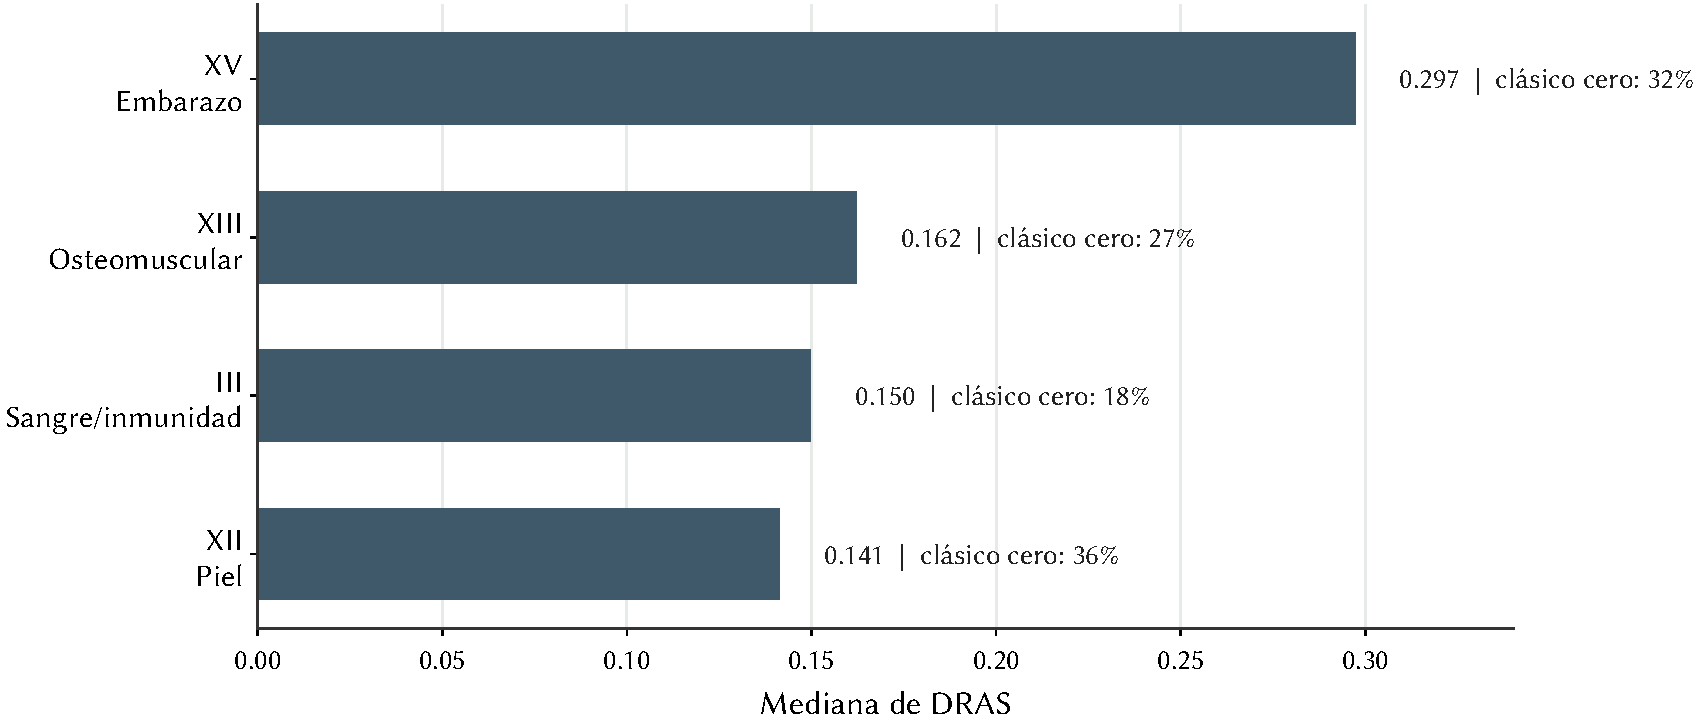
\includegraphics[height=0.41\paperheight,width=\linewidth,keepaspectratio]{dras_celdas_fragiles.pdf}
      \chartnote{DRAS: Diferencia Relativa Absoluta Simétrica; la etiqueta reporta el porcentaje de \(q\) clásico igual a cero.}{Elaboración propia con base en las estimaciones del proyecto.}
    \end{column}
    \begin{column}{0.32\textwidth}
      \RaggedRight
      \vspace{2mm}
      {\large\bfseries Clásico}

      \vspace{1mm}
      {\normalsize \(D_{x,t}^{(c)}=0\)}

      {\normalsize \(\qdec=0\)}

      \vspace{6mm}
      {\large\bfseries Bayes}

      \vspace{1mm}
      {\normalsize suaviza celdas\\ con pocos eventos}
    \end{column}
  \end{columns}
  \note{Benjamín. La comparación de enfoques no se usa para decir que uno es siempre mejor. La lectura es más fina: en la mayoría de celdas con suficiente información, clásico y bayesiano son cercanos. Las diferencias aparecen cuando hay pocos eventos, dominios restringidos o muchos ceros clásicos. La DRAS sube en embarazo, causas osteomusculares, sangre e inmunidad y piel, pero las diferencias absolutas en \(q_{x,t}^{(c)}\) son muy pequeñas. El mensaje es que Bayes suaviza celdas sensibles sin cambiar la historia general.}
\end{frame}

\begin{frame}{El alcance depende del periodo y de la calidad del registro}
  \vspace{8mm}
  \centering
  \limitpoint{Datos agregados}{sin trayectorias}
  \hfill
  \limitpoint{2015-2018}{período corto}
  \hfill
  \limitpoint{Registro}{calidad desigual}

  \vspace{9mm}
  {\large\bfseries Próximo paso: más años, incertidumbre y mejores exposiciones}

  \note{Benjamín. Esta filmina evita sobreprometer. El resultado es útil, pero está delimitado. Trabajamos con datos agregados, no trayectorias individuales; con una ventana corta, 2015 a 2018; y con registros de mortalidad que pueden variar en calidad entre países. Las extensiones naturales son ampliar la serie temporal, incorporar intervalos de incertidumbre de forma sistemática y revisar con más detalle la calidad demográfica de las exposiciones. Con esto dejamos preparado el cierre.}
\end{frame}

\begin{frame}{La causa organiza una lectura más útil que el total}
  \vspace{3mm}
  {\fontsize{14}{16}\selectfont\bfseries
  Los decrementos múltiples muestran dónde cambia el riesgo, cómo se reparte la mortalidad y cuándo conviene suavizar celdas frágiles.}

  \vspace{5mm}
  \closingpoint{mutedteal}{Hombres jóvenes}{La señal externa es más fuerte\\en \mbox{El Salvador}.}
  \hfill
  \closingpoint{mutedbrown}{Edades avanzadas}{La mortalidad circulatoria gana peso y varía por país.}
  \hfill
  \closingpoint{mutedblue}{Celdas escasas}{Bayes suaviza celdas pequeñas sin cambiar la lectura general.}

  \vspace{5mm}
  {\large\bfseries Conclusión: no basta contar defunciones; hay que leer causa, edad y población.}

  \note{Benjamín. Cierre. Volvemos a la pregunta del informe. El total de defunciones no basta para leer la mortalidad centroamericana. Las causas externas pesan más en hombres jóvenes, las enfermedades circulatorias ganan peso en edades avanzadas y el suavizamiento bayesiano ayuda en celdas con pocos eventos sin modificar la lectura general. La conclusión es que la desagregación por causa, edad, sexo y país no es un detalle técnico: es lo que permite interpretar el fenómeno.}
\end{frame}

\begin{frame}[t,noframenumbering]{Referencias}
  \vspace{-5.8mm}
  \begingroup
  \RaggedRight
  \begin{list}{}{%
    \setlength{\leftmargin}{-5.5mm}%
    \setlength{\rightmargin}{-5.5mm}%
    \setlength{\topsep}{0pt}%
    \setlength{\partopsep}{0pt}%
    \setlength{\parsep}{0pt}%
    \setlength{\itemsep}{0pt}%
  }
  \item[]\fontsize{6.7}{7.25}\selectfont
  \aparef{Bowers, N. L., Gerber, H. U., Hickman, J. C., Jones, D. A., \& Nesbitt, C. J. (1997). \textit{Actuarial mathematics} (2nd ed.). Society of Actuaries.}
  \aparef{Calazans, J. A., \& Queiroz, B. L. (2020). The adult mortality profile by cause of death in 10 Latin American countries (2000-2016). \textit{Revista Panamericana de Salud Pública, 44}, e1. \url{https://doi.org/10.26633/RPSP.2020.1}}
  \aparef{Deshmukh, S. (2012). \textit{Multiple decrement models in insurance: An introduction using R}. Springer. \url{https://doi.org/10.1007/978-81-322-0659-0}}
  \aparef{Fine, J. P., \& Gray, R. J. (1999). A proportional hazards model for the subdistribution of a competing risk. \textit{Journal of the American Statistical Association, 94}(446), 496-509. \url{https://doi.org/10.1080/01621459.1999.10474144}}
  \aparef{Goerlich Gisbert, F. J. (2012). \textit{Tablas de vida de decrementos múltiples: Mortalidad por causas en España (1975-2008)} (Documento de Trabajo No. 1/2012). Fundación BBVA.}
  \aparef{Keyfitz, N., Preston, S. H., \& Schoen, R. (1972). Inferring probabilities from rates: Extension to multiple decrement. \textit{Scandinavian Actuarial Journal, 1972}(1), 1-13. \url{https://doi.org/10.1080/03461238.1972.10404630}}
  \aparef{Macdonald, A. S., \& Richards, S. J. (2025). On contemporary mortality models for actuarial use II: Principles. \textit{British Actuarial Journal, 30}, e19. \url{https://doi.org/10.1017/S1357321725000133}}
  \aparef{Manton, K. G., Woodbury, M. A., Stallard, E., Riggan, W. B., Creason, J. P., \& Pellom, A. C. (1989). Empirical Bayes procedures for stabilizing maps of U.S. cancer mortality rates. \textit{Journal of the American Statistical Association, 84}(407), 637-650. \url{https://doi.org/10.1080/01621459.1989.10478816}}
  \aparef{Olivieri, A., \& Pitacco, E. (2012). Life tables in actuarial models: From the deterministic setting to a Bayesian approach. \textit{AStA Advances in Statistical Analysis, 96}, 127-153. \url{https://doi.org/10.1007/s10182-011-0177-y}}
  \aparef{Pitacco, E., Denuit, M., Haberman, S., \& Olivieri, A. (2009). \textit{Modelling longevity dynamics for pensions and annuity business}. Oxford University Press. \url{https://doi.org/10.1093/oso/9780199547272.001.0001}}
  \aparef{Schmitt, F. O., Gilardoni, G. L., \& Andrade, J. A. A. (2019). A class of flat prior distributions for the Poisson-gamma hierarchical model. \textit{Statistica Neerlandica, 73}(3), 414-433. \url{https://doi.org/10.1111/stan.12176}}
  \aparef{Schumacher, A. E., McCormick, T. H., Wakefield, J., Chu, Y., Perin, J., Villavicencio, F., Simon, N., \& Liu, L. (2022). A flexible Bayesian framework to estimate age- and cause-specific child mortality over time from sample registration data. \textit{The Annals of Applied Statistics, 16}(1), 124-143. \url{https://doi.org/10.1214/21-AOAS1489}}
  \aparef{Society of Actuaries. (2016). \textit{Experience study calculations}.}
  \aparef{United Nations, Department of Economic and Social Affairs, Population Division. (2024). \textit{World population prospects 2024}. \url{https://population.un.org/wpp/}}
  \aparef{Wolbers, M., Koller, M. T., Stel, V. S., Schaer, B., Jager, K. J., Leffondré, K., \& Heinze, G. (2014). Competing risks analyses: Objectives and approaches. \textit{European Heart Journal, 35}(42), 2936-2941. \url{https://doi.org/10.1093/eurheartj/ehu131}}
  \aparef{World Health Organization. (2026). \textit{WHO Mortality Database}. \url{https://www.who.int/data/data-collection-tools/who-mortality-database}}
  \end{list}
  \endgroup
\end{frame}

\end{document}
